\chapter{Analysis Optimization}\label{sec:analysis_optimization}
After a thoughtful design of physical objects that correspond to the final state of the process of interest the main task remains to construct some quantity to compare the prediction with the observation. Usually this is done with some kinematic variable e.g. in this analysis it could be the invariant mass of the Higgs pair system $m_\text{HH}$ designed to differentiate signal from background. Events are then counted with a histogram for this variable to be then tested on the statistical significance of an hypothesis.

Since the purpose of this quantity is to classify it is actually better suited to be treated with a \ac{ml} model as already applied widely in particles physics \citep{albertsson2019machine,shlomi2020graph,feickert2021living,Schwartz2021Modern}. However a key issue with any optimization or \ac{ml} model used in a typical particle physics analysis is that it is not optimized for the actual final quantity of interest like a discovery significance or the level of confidence if a tested hypothesis should be accepted or rejected. Usually optimization is done with some ratio of signal to background or in the case of \ac{ml} models by optimizing on the best separation of signal and background(s).

Even though the signal to background ratio or the separation power of the \ac{ml} model is correlated in some way to the expressivity of the statistical test it is not optimal and in particular does not account for uncertainties that can crucially influence the result of the statistical test. This means if the statistical test performs very well on the nominal values it is trained or tested on its behavior can change dramatically if given inputs that deviate from the nominal values (uncertainties) and the power of the statistical test degrades accordingly.

This issue can be addressed with: \textit{\ac{neos}} \citep{Simpson_2023}. It is based on the observation that the classifier training can be done with respect to the actual final quantity of interest by including the statistcal model into the training.


\section{Machine Learning}
\ac{ml} refers to algorithms that enable computers to learn from data to make predictions for some specific task without being explicitly programmed for \citep{kubat2021introduction}. One particular subset of \ac{ml} are \acp{ann} inspired by the human brain. Their fundamental unit are nodes, the neurons, that are interconnected to several other neurons organized in consecutive layers with an initial input and a desired output as shown in figure \ref{fig:ann}. The signals between neurons are transferred weighted and each neuron has an activation function that converts the received input stimulus into an output strength. Thus learning occurs through adjusting the weights between the neurons. \acp{ann} can be designed in various ways with many hidden or deep layers depending on the specific task.
\begin{figure}
    \centering
    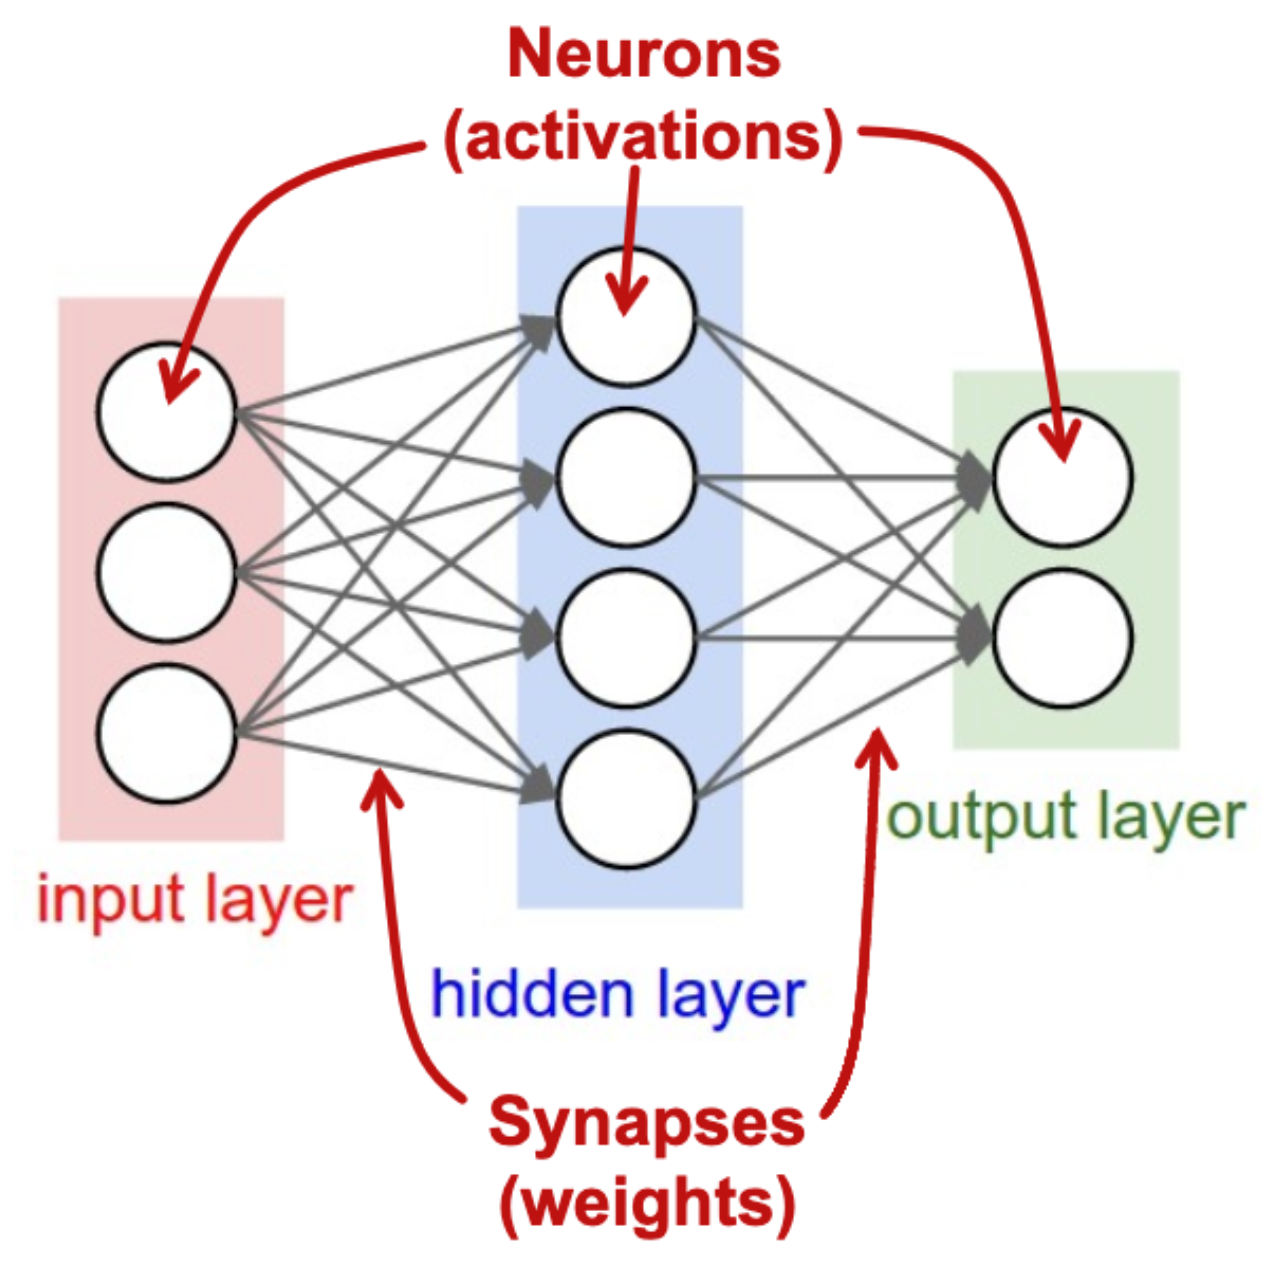
\includegraphics[width=0.4\textwidth]{ann}
    \caption[]{Structure of artificial feed-forward neural networks. Adopted from \citep{8114708}.}
    \label{fig:ann}
\end{figure}

The training of \acp{nn} is usually done with the back-propagation algorithm which seeks to minimize a cost function $C(\bm{\varphi})$ that is designed to measure the deviance of a presented input to a desired output dependent on the model parameters $\bm{\varphi}$. For a feed-forward \ac{nn} these model parameters are the mentioned weights of the neurons. Via gradient descent the minimum of the cost function can be found stepwise with the first derivative and a chosen learning rate parameter $\gamma$
\begin{equation}
    \bm{\varphi}_{n+1} = \bm{\varphi}_n-\gamma\nabla C(\bm{\varphi}_n).
    \label{eq:grad_descent}
\end{equation}
In three dimensions this corresponds to a mountaineer searching for the valley by going in the direction of the steepest crescent with a stepsize proportional to $\gamma$.



\section{NEOS}
The key idea of \ac{neos} is now to choose the cost function as the quantity which is to be minimized. In this case the $\mathrm{CL}_s$ value is a reasonable choice as discussed section \red{\ref{sec:statistics}}. For a typical analysis chain as shown in figure \ref{fig:neos} this corresponds mathematically to a functional concatenation of the individual steps in the chain, as each step depends on the previous one.
\begin{figure}
    \centering
    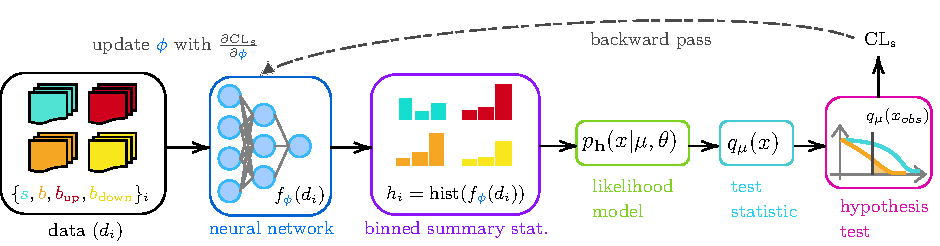
\includegraphics[width=1\textwidth]{neos}
    \caption[]{Typical particle physics analysis chain. For \ac{neos} the $\text{CL}_s$ value is back-propagated to train the neural network parameters  $\bm{\varphi}$. Adopted from \citep{Simpson_2023}.}
    \label{fig:neos}
\end{figure}
Hence the cost function $\text{CL}_s$ is a function of the Dataset $\mathcal{D}$ and the \ac{ml} model parameters $\bm{\varphi}$
\begin{equation}
    \mathrm{CL}_s = f(\mathcal{D},\bm{\varphi}) = (f_{\mathrm{sensitivity}} \circ f_{\mathrm{test\,stat}} \circ f_{\mathrm{likelihood}}  \circ f_{\mathrm{histogram}}  \circ f_{\mathrm{observable}})(\mathcal{D},\bm{\varphi}).
\end{equation}
In order to find the minimum via the gradient descent of equation \ref{eq:grad_descent} \cls needs to be differentiable with respect to $\bm{\varphi}$. By applying the chain rule this reads for one model parameter $\varphi_i$
\begin{equation}
    \frac{\partial\,\mathrm{CL}_s}{\partial \varphi_i} = \frac{\partial f_{\mathrm{sensitivity}}}{\partial f_{\mathrm{test\,stat}}}\frac{\partial f_{\mathrm{test\,stat}}}{\partial f_{ \mathrm{likelihood}}} \frac{\partial f_{\mathrm{likelihood}}}{\partial f_{\mathrm{histogram}}}   \frac{\partial f_{\mathrm{histogram}}}{\partial f_{\mathrm{observable}}}  \frac{\partial f_{\mathrm{observable}}}{\partial \varphi_i}.
\end{equation}
Apart from histogramming which is inherently discrete all steps are differentiable. One way to make histograms differentiable is \ac{kde} \citep{CRANMER2001198}. Instead of counting a quantity in bins, a histogram can be approximated by representing each data point by a normal distribution, the kernel, with the mean of the data point and a chosen value for the standard deviation, also called the bandwidth in this context. Since the area under the Gaussian is equal to one, the summation of all Gaussian's can produce a smoothed estimate of a histogram that is inherently differentiable. However the bandwidth should be chosen around the desired binning width as the estimate depends crucially on it, as exemplified in Figure \ref{fig:relaxed_hist}. Although this can be a source of uncertainty one can always revert any differentiable step or block in figure \ref{fig:neos} and go back to the exact calculation.
\begin{figure}
    \centering
    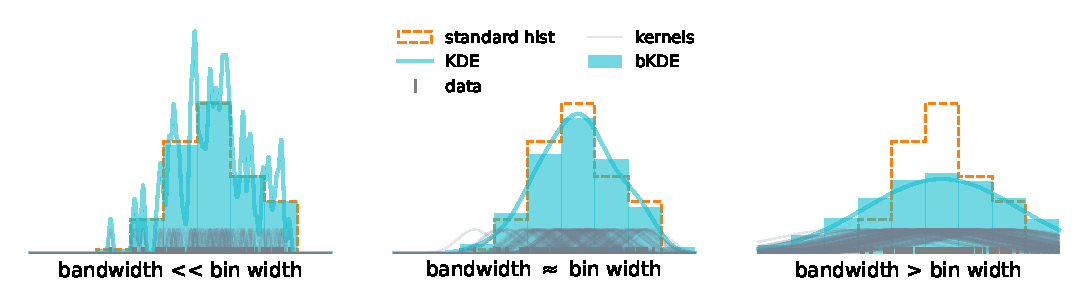
\includegraphics[width=1\textwidth]{relaxed_hist}
    \caption[]{Dependence of the histogram approximation with normal distributions of different standard deviations called bandwidth in the context of \ac{kde}. Depicted in grey small bars on the x-axis are the data points and their kernel estimates above them, the standard histogram binned from data, the \ac{kde} and the \ac{bkde} as a histogram resulting from the \ac{kde}. Adopted from \citep{Simpson_2023}.}
    \label{fig:relaxed_hist}
\end{figure}

\subsection{Implementation}
To trace the differentiation through software is again achieved with a simple observation that in fact any software is only a concatenation of elementary arithmetic operations. Since their analytic solutions are known all there is to do is the concatenate of all these operations and differtiate this function to calculate. This is also known as \textit{Automatic Differentiation} and is achieved here with the help of the software package \textsc{jax} \citep{jax2018github}.

Although the idea seems simple and one of the reasons it has not been attempted previously is that it can be conceivably difficult to differentiate through multiple individual software frameworks. That this became feasible in a reasonable time-frame builds on the efforts to port the individual steps to the \textsc{python} programming language away from C++ \textsc{root}-based software \citep{ANTCHEVA20092499}. While \textsc{root} was indispensable at its time of emergence it is currently suboptimal for contemporary scientific analysis. This is because it is not only difficult to integrate within other software but also comparatively user-unfriendly compared to readily available \textsc{python} solutions maintained by a scientific community doing data-analysis. Using \textsc{python} in this context presents a notable advantage since many problems have already been addressed and instead of relying on a small group for maintenance there is support from a large community. This enables out-of-the-box applications as for example the use of \textsc{jax} which a priori has no connection to \ac{hep}. 

The original proposers \citet{Simpson_2023} of \ac{neos} developed differentiable versions of common \ac{hep} tasks like the upper mentioned hypothesis test, histogramming and the optimization of a cut in a packaged called \textsc{relaxed} \citep{Simpson_relaxed_version_0_3_0_2023}. Using this they tested the whole pipeline successfully in a toy model \citep{Simpson_neos_version_0_2_0_2021}. These efforts were transferred and further developed to be applicable to this analysis with \citep{hh_neos}. \red{how about a better repo name: sensitivo, sensitivity optimizer?}
